\chapter{Fundamentos geodésicos e cartográficos}

Como os SIG herdam conceitos utilizados anteriormente na elaboração de mapas, é necessário conhecer esses fundamentos para fazer bom uso das ferramentas que um SIG oferece. Nesse sentido, os elementos da geodésia e da cartografia são fundamentais, pois sem eles não é possível compreender o contexto de um SIG.

\section{Conceitos geodésicos básicos}
\pagestyle{fancy}

A principal característica da informação georreferenciada é que ela possui uma \textbf{localização no espaço}, particularmente no espaço terrestre. Essa localização deve ser expressa por meio de \textbf{coordenadas}, o que exige o estabelecimento de um sistema apropriado para tal. 

A \textbf{geodésia} é a ciência que fornece a base teórica para isso e tem como objeto de estudo \textbf{a forma da Terra}. Através de seus diversos ramos, a geodésia oferece métodos e conceitos que permitem o uso rigoroso de coordenadas.

A necessidade da geodésia surge do fato de que a Terra não é plana. Quando se trabalha com áreas suficientemente extensas, sua curvatura não pode ser ignorada. Esse é o caso típico em um SIG, e por isso os SIG implementam os elementos necessários para lidar rigorosamente com a informação geográfica, conforme os conceitos geodésicos.

Um dos principais objetivos da geodésia é estabelecer um sistema de referência e definir um conjunto de pontos (conhecidos como \textbf{vértices geodésicos}) cujas coordenadas nesse sistema sejam conhecidas com elevada precisão. A partir desses pontos, que formam uma \textbf{rede geodésica}, é possível calcular as coordenadas de qualquer outro ponto no sistema de referência.

\subsection{Superfícies de referência}

Dois conceitos básicos são fundamentais aqui: o \textbf{elipsoide de referência} e o \textbf{geoide}.

A Terra possui forma esferoide, mas não é uma esfera perfeita: é achatada nos polos, formando um \textbf{elipsoide}. Nesse modelo, o raio da Terra varia com a localização. Assumir a Terra como um elipsoide é mais preciso do que considerá-la perfeitamente esférica, sendo essencial na elaboração de cartografia de áreas extensas.

Após definir teoricamente a forma da Terra, é necessário determinar os parâmetros que a caracterizam. Para uma esfera, calcula-se o raio. Para um elipsoide, determinam-se os comprimentos dos semieixos maior e menor.

Por razões históricas, existem diversos elipsoides definidos por geodestas ao longo do tempo e em diferentes regiões. Os primeiros elipsoides de uso global surgiram há cerca de um século com o intuito de criar uma referência internacional. O \textbf{elipsoide WGS--84} é atualmente um dos mais utilizados, sendo adotado pelo sistema GPS.

O \textbf{geoide} é outra superfície de referência, definida como a superfície tridimensional em que a força da gravidade é constante. Corresponde a uma superfície equipotencial obtida ao se imaginar os oceanos em repouso e em nível médio, estendendo-se por baixo da superfície terrestre.

Assim como os elipsoides, há diversos geoides de referência, que evoluem ao longo do tempo para se adaptar às mudanças na superfície da Terra.

A Figura~\ref{Fig:Tres_superficies} apresenta uma comparação esquemática entre as três superfícies: a real, o geoide e o elipsoide.

\begin{figure}
\centering
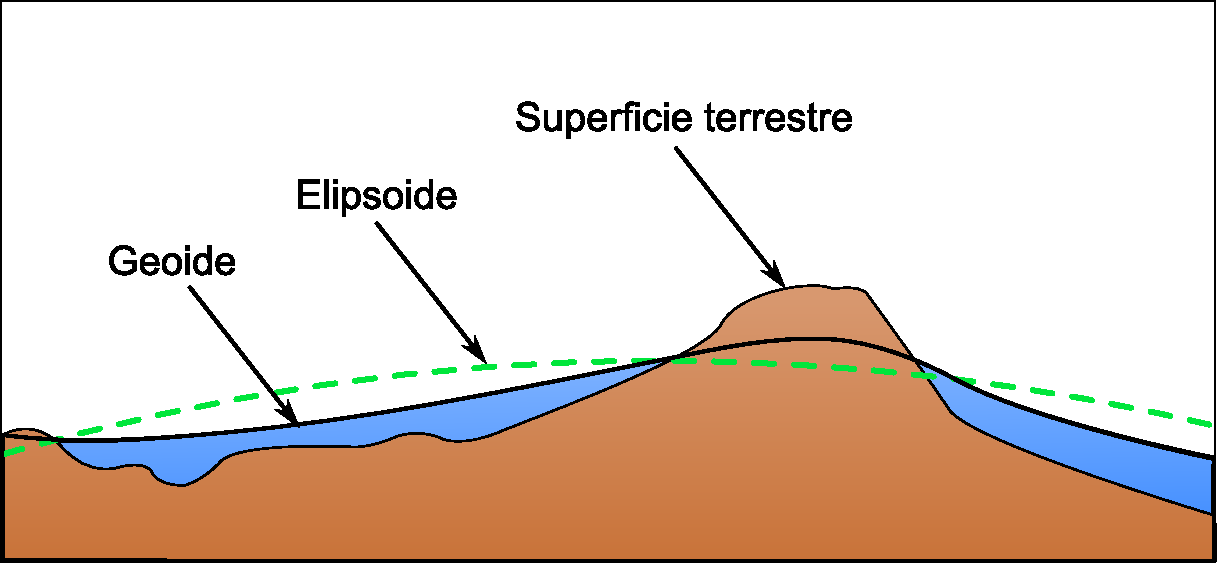
\includegraphics[width=.7\columnwidth]{Fundamentos_cartograficos/Tres_superficies.pdf}
\caption{\small Três superfícies fundamentais: superfície real da Terra, geoide e elipsoide (Adaptado da Wikipédia).}
\label{Fig:Tres_superficies} 
\end{figure}

Num elipsoide \textbf{global}, tanto o centro de gravidade quanto o plano equatorial coincidem com os da Terra. Já num elipsoide \textbf{local}, essas coincidências não são garantidas, sendo necessário mais informação sobre sua posição em relação à superfície terrestre.

Surge então o conceito de \textbf{datum}, que é a combinação de uma superfície de referência (elipsoide) e um ponto que o conecta ao geoide. Esse ponto é chamado de \textbf{ponto fundamental}, onde o elipsoide é tangente ao geoide. As verticais do geoide e do elipsoide coincidem nesse ponto.

Para um mesmo elipsoide, diferentes pontos fundamentais originam diferentes datums e, portanto, diferentes coordenadas para um mesmo ponto.

\subsection{Sistemas de coordenadas}

Após definir um modelo para a forma da Terra, podemos estabelecer um sistema para codificar posições em sua superfície e atribuir coordenadas a cada ponto. Há duas opções principais: utilizar \textbf{geometria esférica} para definir um sistema de coordenadas esféricas, ou utilizar \textbf{geometria plana}, o que exige uma \textbf{projeção cartográfica} da superfície curva para um plano.

O sistema de \textbf{coordenadas geográficas} é baseado em esferas, localizando pontos por meio de dois valores angulares: \textbf{latitude} e \textbf{longitude}. As linhas de mesma latitude e longitude são chamadas de \textbf{paralelos} e \textbf{meridianos}, respectivamente.

As coordenadas geográficas são muito úteis para grandes áreas, mas não constituem um sistema cartesiano. Tarefas como \textbf{medição de áreas ou distâncias} são complicadas com elas. Para facilitar tais operações e gerar cartografia, utilizamos coordenadas cartesianas, obtidas por meio da \textbf{projeção cartográfica}.

Como a superfície da esfera não é \textbf{desenvolvível} (isto é, não pode ser transformada em plano sem distorções), é necessário um método para converter seus pontos a um plano, conforme ilustra a Figura~\ref{Fig:Proyeccion}.

\begin{figure}
\centering
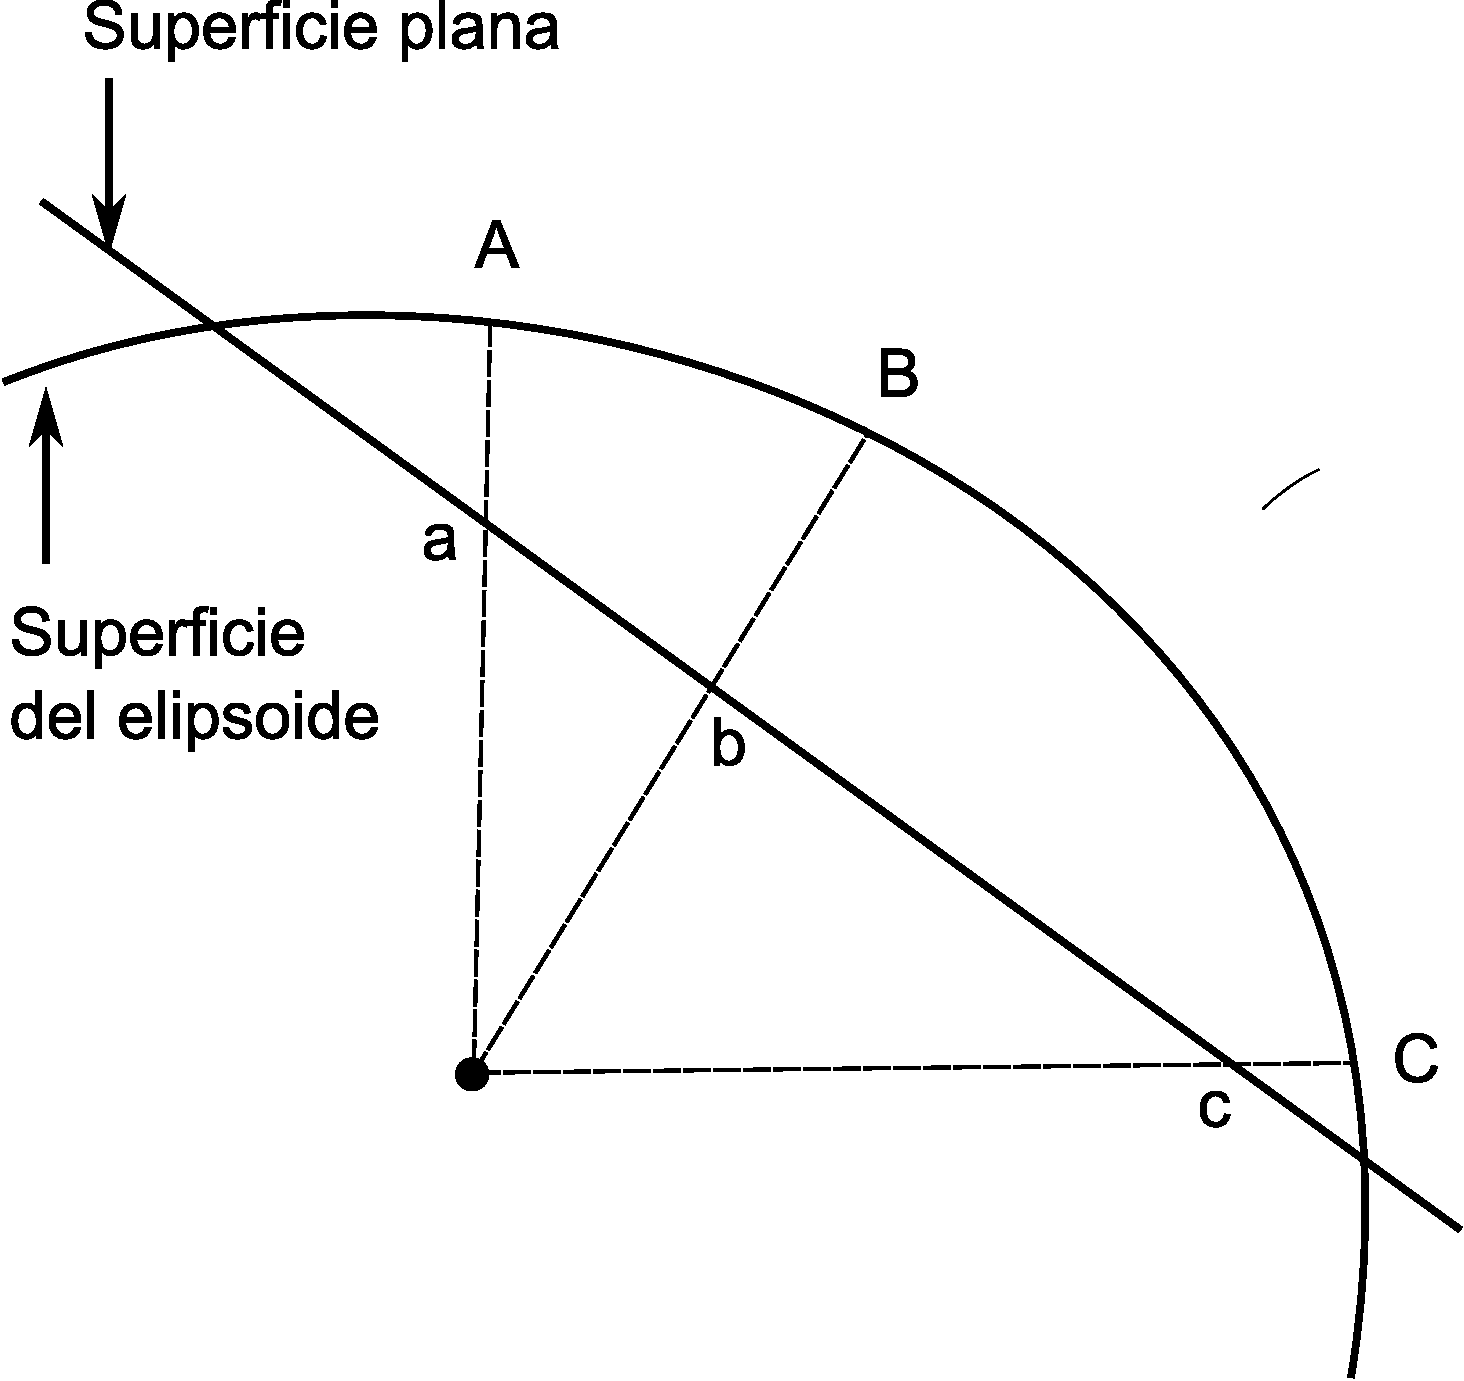
\includegraphics[width=.5\columnwidth]{Fundamentos_cartograficos/Proyeccion.pdf}
\caption{\small Esquema do conceito de projeção. Os pontos $A, B$ e $C$ na superfície do elipsoide têm equivalentes $a, b$ e $c$ no plano.}
\label{Fig:Proyeccion} 
\end{figure}

Além da projeção direta sobre um plano, pode-se usar superfícies desenvolvíveis, como cilindros ou cones, originando \textbf{projeções cônicas} ou \textbf{cilíndricas}.

Como mostra a figura, todas as projeções produzem \textbf{distorções}, chamadas de \textbf{anamorfoses}. A distância entre $A$ e $B$ na superfície não é igual à entre $a$ e $b$ no plano.

Conforme as propriedades métricas que preservam, as projeções podem ser:

\begin{itemize}
 \item \textbf{Equiárea} — preservam áreas;
 \item \textbf{Conformes} — preservam ângulos e formas;
 \item \textbf{Equidistantes} — preservam distâncias.
\end{itemize}

A escolha da projeção depende das \textbf{necessidades específicas} da aplicação.

Atualmente, uma das mais utilizadas é a \textbf{projeção transversa de Mercator}, que dá origem ao \textbf{sistema de coordenadas UTM}. Esse sistema divide a Terra em zonas e aplica parâmetros geodésicos específicos a cada uma. Usa o elipsoide WGS--84.

No sistema UTM, as coordenadas são expressas por meio de \textbf{zona + coordenadas relativas}. A Terra é dividida em 60 \textbf{fusos} de 6° de longitude cada, numerados de 1 a 60, de oeste para leste. Cada fuso é subdividido em 20 zonas latitudinais (C a X, exceto I e O), cada uma com 8° de latitude, exceto a zona X (12°).

As coordenadas são dadas em metros, com origem no cruzamento entre o meridiano central do fuso e o equador. Para evitar valores negativos, define-se a coordenada X inicial como 500.000 m, e a Y como 10.000.000 m (no hemisfério sul).

\subsection{Transformação e conversão de coordenadas}

É comum em SIG lidar com \textbf{diferentes sistemas de coordenadas} ou datums. Para unificar a informação, torna-se necessário \textbf{converter} os dados para um sistema comum. Se os datums forem diferentes, falamos em \textbf{transformação de coordenadas}.

SIGs oferecem funcionalidades para modificar as coordenadas dos dados geográficos ou para representá-los \textbf{em tempo real} em outro sistema (conversão \emph{on-the-fly}).

Sistemas de referência são padronizados com códigos. O mais comum é o \textbf{EPSG}.

\section{Conceitos cartográficos básicos}

Entre os conceitos fundamentais da cartografia destaca-se a \textbf{escala}, que expressa a \textbf{relação de tamanho} entre a representação no mapa e a realidade. Com ela, podemos converter medições do mapa em valores reais.

A escala é expressa como uma razão, por exemplo, 1:50.000 significa que 1 cm no mapa representa 500 m na realidade — isso é a \textbf{escala numérica}.

A escala só é exata em certas partes do mapa. Fora delas, varia. A razão entre a escala local e a numérica é o \textbf{fator de escala}.

Embora associada à representação, a escala também está ligada à \textbf{resolução dos dados} — ou seja, ao \textbf{tamanho mínimo cartografado} —, o que define a chamada \textbf{escala operacional} dos dados.

Em SIG, é possível aumentar a escala de visualização (\textbf{escala cartográfica}), mas isso não revela mais detalhes. Para isso, seria necessário coletar novos dados.

No caso de dados \emph{ráster}, o parâmetro relevante é o \textbf{tamanho da célula}, relacionado à escala.

O conceito de \textbf{generalização cartográfica} está ligado à representação simplificada de dados. É essencial para representar dados em escalas menores do que a escala de coleta. A Figura~\ref{Fig:Generalizacion_agregacion} mostra um exemplo.

\begin{figure}[!hbt]
\centering
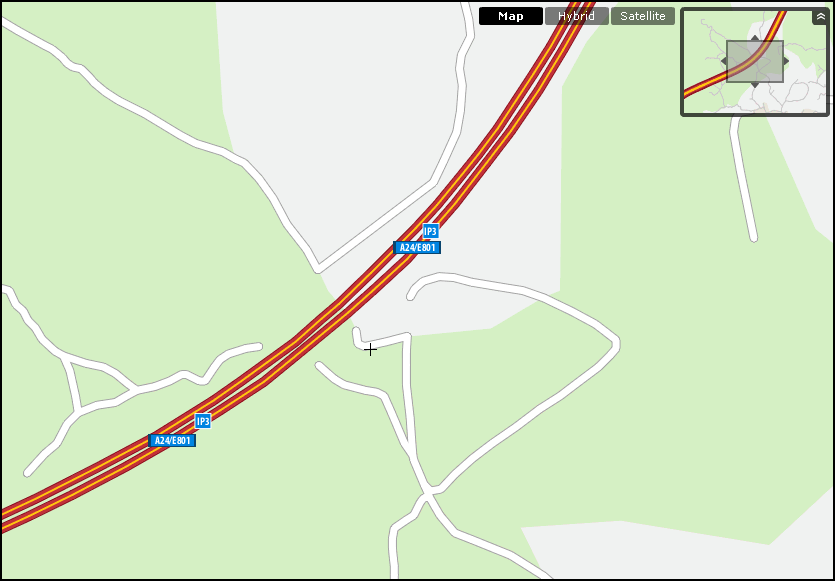
\includegraphics[width=.75\columnwidth]{Fundamentos_cartograficos/Generalizacion_agregacion.png}
\caption{\small Exemplo de generalização por agregação. Duas vias paralelas representadas como uma única via em escala menor (Fonte: Yahoo Maps).}
\label{Fig:Generalizacion_agregacion} 
\end{figure}

Outras operações de generalização incluem: 
\textbf{simplificação}, \textbf{agregação}, \textbf{exageração} (aumentar tamanho), e \textbf{deslocamento} (ajustar posição para legibilidade).

Em SIGs, a generalização pode ser feita em tempo real, mas isso consome muitos recursos e pode gerar resultados ruins.

Uma alternativa melhor é o uso de um \textbf{modelo multi-escalar} (Figura~\ref{Fig:SIG_multi_escala}), onde se mantém versões dos dados em diferentes escalas.

\begin{figure}[!hbt]
\centering
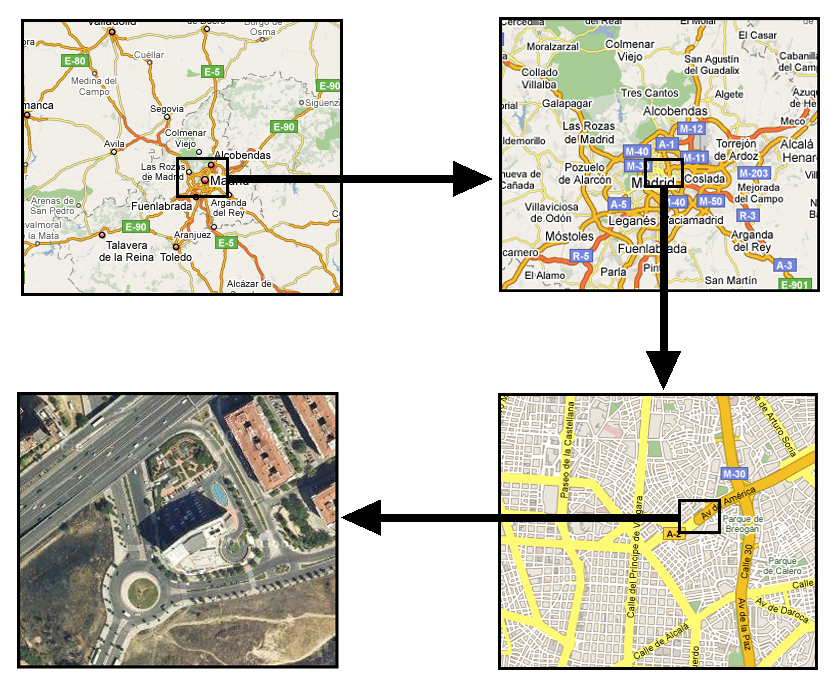
\includegraphics[width=\textwidth]{Fundamentos_cartograficos/SIG_multi_escala.png}
\caption{\small Em um SIG, é comum trabalhar com dados em diferentes escalas. A informação exibida depende da escala.}
\label{Fig:SIG_multi_escala} 
\end{figure}

O conceito de \emph{camada}, fundamental em SIGs, permite gerenciar dados em múltiplas escalas.

Para imagens, isso se traduz na criação de \textbf{pirâmides}, ou seja, conjuntos de imagens em diferentes resoluções, escolhidas conforme a escala de visualização.

\pagestyle{empty}
